\documentclass{article}

\usepackage{url}
\usepackage{spconf,amsmath,graphicx}
\usepackage{amsmath}
\usepackage[linesnumbered,ruled]{algorithm2e}
\usepackage{float}
\usepackage{stfloats}
\usepackage{caption}
\usepackage{amsmath}
\usepackage{verbatim}

% Example definitions.

% --------------------
\def\x{{\mathbf x}}
\def\L{{\cal L}}

% Title.

% ------
\title{A Game Prediction Algorithm for Dota}
%
% Single address.

% ---------------
\name{Runzhou Cao, Xiaohu Zhao, Fang Zhou}
\address{The Ohio State University}
%
% For example:
% ------------
%\address{School\\
%	Department\\
%	Address}
%
% Two addresses (uncomment and modify for two-address case).

\begin{document}
%\ninept
%
\maketitle
%
\begin{abstract}
Dota is one of the most popular eSports because of its high entertainment.
There are only few machine learning algorithms for Dota game prediction.
The exisiting research faces several problems so that the results cannot
be reliable.

In this paper, we design a new algorithm for Dota game prediciton.  
First, we design a comprehensive feature vector used in the machine learning algorithms.
Second, we try different machine learning algorithms to choose the best one.
Last but not least, the data scale in our experiments is so large that the results can be reliable.
The results show our algorithm is both effective and efficient.

\end{abstract}
\begin{keywords}
Machine Learning, Dota, eSports, Predition, Decision Tree.
\end{keywords}
%
\section{Introduction}

ESports, also known as electronic sports, has become an official sport since the 21st century.
The new technologies applied in the eSports are attractive to the young and old.
The 3D graphic display, vivid sound effect, immersive experience, and the interesting operations make eSports more and more popular.
According to a report~\cite{esports}, In 2013, it was estimated that approximately 71.5 million people worldwide watched eSports.

Since eSports games are increasingly popular, the prediction of eSports game result has become increasingly significant.
The estimation of game results can be used to train the professional players at ordinary times and modify the gamer’s tactic for the upcoming game.
This estimation can also be used for media.
In addition, the predictions of the game results can improve the entertainment for fans.

Therefore, we decide to design and implement a prediction system based on machine learning technology for eSports games.
In this paper, we focus on the one of the most popular eSports games is Dota.
Dota is the short name for Defense of the Ancients.
Dota~\cite{dotablog} is a free-to-play multiplayer online battle arena video game.
Two five-player teams compete in the playing field, where each player chooses one from a total of 111 heroes to play.
Millions of game players take part in Dota every day.
With the highly-speed development of eSports, abundant and grand eSports competitions are organized globally every month, season, and year.
Prize pool of millions of dollars is often provided by some competitions.

Prior research 
Conley et al.~\cite{conley2013does} did a research on which machine learning method is the best for data game results.
However, they only focus on two machine learning approaches, linear regression and k-nearest neighbour(kNN).
Kalyannaraman~\cite{kau2013win} did an augmented algorithm on traditional linear regression considering pair relationships of heroes.
However, he did not consider all the relationship between heroes, like the restraint relationship between heroes.
What's more, these two research did not test on large scale of data, which means not so reliable on their results.
Drachen et al. ~\cite{drachen2014skill} try to predict the temporal and spatial of players in the game based on the hero skills.
But the objective is different from ours. 

Our goal is to predict the results of Dota Game.
It means, given the specific two groups of heroes, we can give back the users the predicted outcome of the game.
In this paper, the contributions include:

\begin{itemize}
\item We are the first one to consider the restraint relationship of heroes into the prediciton of Dota game result. 
\item We are the first one to introduce the game lasting time as a feature vector in the prediction. 
\item We abstract the Dota game prediction problem and applied different machine learning approaches.
\item Through tuning the parameters in the machine learning approaches, we compare the performance among different algorithms. We also conclude the results and analyze the results.
\end{itemize}

The rest of the paper proceeds as follows.
Section 2 introduces Dota and mainstream machine learning algorithms we try in this paper.
Section 3 gives a brief introduction about the abstract of the problem and the goal.
Then in the section 4, we talk about the design of our machine learning algorithms; also a detailed description of Decision Tree is given.
In the section 5, we will describe our data sets, training and testing methods, evaluation metrics and results.
Section 6 introduces some related papers.
In the final section, we will analyze the results of the prediction.

\section{Background}
In this section, we first introduce Dota game.
Then, we continue to introduce the meachine learning algorithms we want to test in this paper. 

\subsection{Dota}
In each dota game, there are two teams against each other.
Each team consists of five players.
Before starting the game, the players one by one choose one hero from the hero pool, which includes 111 heroes in total.
Different heroes has different skills and play different roles in the team.
The buildings in the game have health points.
The final objective of Dota is to destory the enemy base, which means they want to make the enemy base's health points become 0. 

Even though different heroes have different skills, we can always classify the heroes into four categories: Carry, Support, Ganker, and Initiator.

\begin{itemize}
\item \textbf{Carry:}
These heroes play the core role in a team.
They are the main attack output of a team.
Usually, there are only one carry in a team.
But sometimes, maybe another carry is picked up in case that the main carry cannot develop very well.
However, at first, these heroes are not good at battle so they need some time to level up.
They usually take over the game in the group battle at the end of a game.
In most cases, all the behaviors of other heores in a team serve for the carry heroes.
For example, other heroes always protect the carry's life and sometimes they choose to die instead of the carry hero.
\item \textbf{Support:} 
The heroes belonging to support, as its name, offers help and support to other heroes.
They need spend much money to buy something useful for the whole team.
For example, they always buy couriers and wards, which help the carry speedup the progression.
The other example is they always buy the eyes to provide views so the team can take advantage before the group battle.
They are very easily ignored because they are very easy to deaths. 
However, they are very hard to play well because they need to keep themselves 
safe and earn little money to support the whole team.
\item \textbf{Ganker:}
This kind of heroes are designed to start a quick regional battle and kill one or two enemies in a short time.
They always have some speical skills and efficient high attack output in a short time.
For example, they may have an invisible skill so when they suddenly appear,
the opponent heroes do not have time to react before they die.
Or they may have a very high attack output in 3 second so they can kill the enemies in sudden.
The players who play gankers need to have a very good view of the game so
they can find the best chance to attack the enemy heroes.
Before the carry can join in the group battle,
gankers need to organize the team and make the enemy heroes
uncomfortable so they cannot farm easily.
\item \textbf{Initiator:}
An initiator is the hero who starts the group battle.
They usually have some skills to make enemy heores dizzy and stun for a while.
After they use the skills, other heores starts to enter the group battle.
The timing is very important if you want to play initiators well.
If you starts the group battle in a bad timing, then all your team maybe die.
The role of initiator is very important so the players play initiator always
have very high speed to press keyboard and very good smell of the group battle.
\end{itemize}

\subsection{Mainstream Meachine Learning Algorithms}

\begin{itemize}
\item \textbf{Decision Tree}
A decision tree is a decision support tool that uses a tree-like graph.
The goal of decison tree is achieve perfect classification with minimal number of decisions.
In the training process, we pickup the most representative features from the feature vectors of the data.
Once we generate the tree, we can easily get the prediciton from the decision tree.
The decision tree is very easy to understand and implmement.
After generating the decision tree, the running time of decision tree is very short,
which means the decision tree is very fast to predict.
However, if the data is very complex, the decision tree cannot get a very high accuracy.
What's more, finding out the optimal decision tree is NP-hard problem.

\item \textbf{Logistic Regression}
In statistics, logistic regression is also called logit regression or logit model
Logistic regression is a regression model where the dependent variable (DV) is categorical.
Logistic regression measures the relationship between the categorical dependent variable and
one or more independent variables by estimating probabilities using a logistic function,
which is the cumulative logistic distribution.
Logistic regression can be seen as a special case of the generalized linear model and thus analogous to linear regression. 
Based on the input, logistic regression can return a linear regression, which can be used for classification.
The output of logistic regression is 0 or 1, because the output of logistic regression is the output fo a logistic function.

\item \textbf{Neural Network}
The goal of the neural network is to solve problems in the same way like the human brain,
although several neural networks are much more abstract.
Neural network is inspired by the neural netowrk in biology.
Neural network includes a lot of neurons connected by axons in different levels.
Modern neural network projects typically work with a few thousand
to a few million neural units and millions of connections,
which is still several orders of magnitude less complex than the
human brain and closer to the computing power of a worm.
Deep learning is a kind of neural network with the advantage of current powerful computations 
and several optimizations.

\item \textbf{SVM}
SVM is short for support vector machine.
An SVM model is a representation of the examples as points in space,
mapped so that the examples of the separate categories are divided
by a clear gap that is as wide as possible.
The most interesting part of SVM is kernel trick.
SVMs can efficiently perform a non-linear classification using what is called the kernel trick,
implicitly mapping their inputs into high-dimensional feature spaces.
Different kernels can lead to different results.
So, kernel is the most imporant for the performance of SVM.
\end{itemize}

\section{Problem Description}
This problem is not only a simple estimation of some electronic games,
but also a prediction for people activities.
The practical world is very complex and versatile.
Plenty of immeasurable and unavoidable factors contribute to the results.
Gamer’s skills, physical and emotional condition and the external environment all play important roles,
but none of them can be quantified.
Our prediction system will exclude these uncertain factors to simplify the problem.

\section{Algorithm Design}
In this section, we wil talk about the desing of the algorithms.
\subsection{Feature Design}
The problem can be simplified to a binary classification problem.
The input is the features of the data sets, and the output is the winner side (the sentinel or the scourge).
The prediction will be conducted before the game.
So available features include hero lineup, hero combination, game time and the game results.
Therefore, features include three parts: 
\begin{enumerate}
\item Hero Lineup (111 * 2 dimensions): There are 111 heroes in the game.
Each team will pick 5 heroes in each game.
Each feature can be 1 or 0, meaning picked or not picked.
Therefore, there are 222 dimensions for hero presentation.
\item Positive Relationship (30 * 2 dimenstions):
In Dota, some heroes can cooperate with each other to increase the attack output.
For example, the hero Ursa and the hero Io are always picked together in the same team.
They can cooperate with each other and give a very high attack output.
We choose the most influential pairs of heroes (30 pairs) for each team in positive relationship.
\item Negative Relationship (30 * 2 dimenstions):
In Dota, some heroes's performance are lower by some other heroes.
When they are in the different teams, one hero always push much pressure on the other hero in the other team.
We choose the most importnat pairs of heroes (30 pairs) for each team in negative relationship.
\item Time (1 dimension):
This feature is used to show how long the game lasts.
\item The Result (1 dimension): 0 or 1, Team A wins or Team B wins.
\end{enumerate}
\subsection{Algorithm Decision}

After attempts of several algorithms, such as Decision Tree, Logistic Regression, Natural Network and SVM, we select Decision Tree as our model.
 

XXX: We need more descriptions why we choose decision tree.


Decision Tree is a tree-like model of decisions to analyze problems.
 The nature of a decision three is decision rules.
 A decision tree about discount is presented in Figure~\ref{fig:ctree}.


\begin{figure}[!htbp]
\centering
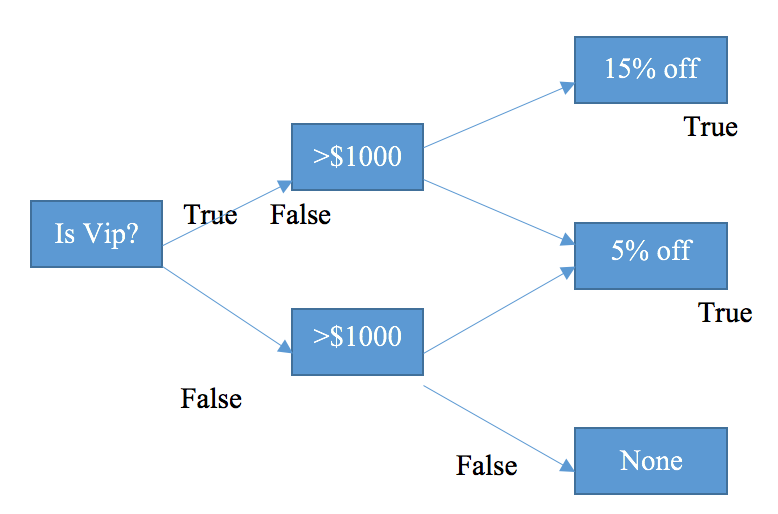
\includegraphics[width=8.0cm]{ctree.png} 
\newline
\caption{An Example of C4.
5 Decision Tree}
\label{fig:ctree} 
\end{figure}

We adopt C4.
5 to generate a decision tree for the problem.
 The algorithm is proposed by Ross Quinlan~\cite{quinlan}, which is an extension of his earlier ID3 algorithm.

The pseudocode~\cite{Kotsiantis} of the general algorithm for building decision trees by C4.
5 is: 

\begin{enumerate}
\item Check for base cases.

\item For each attribute a, find the normalized information gain ratio from splitting on a.

\item Let a\_best be the attribute with the highest normalized information gain.

\item Create a decision node that splits on a\_best.

\item Recur on the sublists obtained by splitting on a\_best, and add those nodes as the children of the node.

\end{enumerate}

\section{Results}
\subsection{Data Sets}
All the data come from Dotabuff, which is the largest third-party Dota2 game track website.
In the team section of Dotabuff, there are more than 1,000 teams sharing their game results.
We write a crawler to collect our data by Python urllib2 and Beautifulsoup libraries.
As Section II mentioned, to keep the balance of the data set, for one game, we generate two feature vectors.
We will first generate one vector based on the original information provided in the website.
Then we will swap the features of two teams to generate the second vector.
We kept running the crawler for four days to collect data.

Our data sets include 15,197 Dota2 matches records from top 100 famous teams in the world.
Each row has 423 features including team ID, hero lineup and result.

\subsection{Training and Testing}
We use 10-fold cross-validation as our training and testing methods.
The original data sets are randomly partitioned into 10 equal sized subsets, use one of the subsets as the test set and the others as the testing set.
The process is to repeate 10 folds, with each subset used exactly once as the testing set.
The results are the combined from 10 folds.


\subsection{Evaluation Metrics}
F-score is used as the evaluation metric our experiment, since both the precision and recall are considered by this method.
F-score can be calculated by the following formulas.


\begin{equation}
F=2\times\frac{Precision+Recall}{Precision*Recall}
\end{equation}

\begin{equation}
Precision = \frac{\#TruePositives}{\#TruePositives+\#FalsePositives}
\end{equation}

\begin{equation}
Recall = \frac{\#TruePositives}{\#TruePositives+\#FalseNegatives}
\end{equation}

We also use Confusion Matrix to present our results.
A sample form is described in Table~\ref{table:sample}.
There are 200 samples in the testing data set.
200 instances are classified correctly, and 100 instances are classified wrongly.

\begin{table}
\begin{center}
\begin{tabular}{|c|c|c|}
\hline
Predicted: True & Predicted: False & N = 200 \\ \hline
100 & 50 & Actual: True \\ \hline
50 & 100 & Actual: False \\ \hline
\end{tabular}
\caption{A Sample of Confusion Matrix}
\label{table:sample}
\end{center}
\end{table}

\subsection{Results}
Due to 10-fold cross-validation, every instance in the data sets has been used as test cases.
There are 15,197 samples in total.
9,247 instances (60.8475\%) have been classified correctly, and 5,950 instances (39.1525\%) have been classified incorrectly.
The accuracy by class and confusion matrix can be seen in Table~\ref{table:accuracy} and Table~\ref{table:matrix}.


\begin{table}
\begin{center}
\begin{tabular}{|c|c|c|c|}
\hline
Class & Precision & Recall & F-score \\ \hline
0 & 0.609 & 0.608 & 0.654 \\ \hline
1 & 0.608 & 0.609 & 0.654 \\ \hline
\end{tabular}
\caption{Detailed Accuracy by Class}
\label{table:accuracy}
\end{center}
\end{table}

\begin{table}
\begin{center}
\begin{tabular}{|c|c|c|}
\hline
a & b & \\ \hline
4,620 & 2,978 & a = 0 \\ \hline
2,972 & 4,627 & b = 1 \\ \hline
\end{tabular}
\caption{Confusion Matrix}
\label{table:matrix}
\end{center}
\end{table}

\subsection{Results from Other Models}
We also applied other models to the problem.
 The results are shown in Table~\ref{table:others}

\begin{table}
\begin{center}
\begin{tabular}{|c|c|}
\hline
Model & F-score \\ \hline
Logistic Regression & 54.08\% \\ \hline
Natural Network & 59.51\% \\ \hline
Support Vector Machine & 60.43\% \\ \hline
Native Bayes & 58.92\% \\ \hline
\end{tabular}
\caption{Results from Other Models}
\label{table:others}
\end{center}
\end{table}

\section{Related Work}
Conley et al.~\cite{conley2013does} did a research on which machine learning method is the best for data game results.
However, they only focus on two machine learning approaches, linear regression and k-nearest neighbour(kNN).
In our paper, we focus on four mainstream machine learning approaches.
Kalyannaraman~\cite{kau2013win} did an augmented algorithm on traditional linear regression considering pair relationships of heroes.
However, he did not consider all the relationship between heroes, like the restraint relationship between heroes.
In our research, we further consider the negative relationship of heroes and the time factor.
What's more, the data scale used in our research is much professional and larger than theirs.
It ensures that our research is more reliable and trusted.

Drachen et al. ~\cite{drachen2014skill} try to predict the temporal and spatial of players in the game based on the hero skills.
Semenov et al. ~\cite{semenovapplications} conclude the current research situation for Dota prediction
and show some opinoins of eSports game prediction.

\section{Conclusion}

This paper proposes a method to predict the eSports game results of Dota.
With three-type features (Team ID, Hero Lineup and Result) and decision tree model, our Dota prediction system gets 65.4\% F-score from a data set of 15,197 matches.
 
The F-score is not relatively high and the reasons are as follows:
\begin{enumerate}
\item Concerning the data sets, we can only get the game records including the information of Team ID, Hero Lineup and result.
More detailed information about teams and games are not available.

\item Regarding features, player’s skills, physical and emotional condition and the external environment all are vital to the result of a game, but none of them can be measured.

\end{enumerate}

% -------------------------------------------------------------------------
\vfill\pagebreak

\bibliographystyle{abbrv}
\bibliography{./Template}

\end{document}
